% Scientific Reports submission manuscript
% Springer Nature LaTeX template, version 3.1 (December 2024)
% Compile with: latexmk -pdf -interaction=nonstopmode -halt-on-error manuscript.tex
\documentclass[pdflatex,sn-nature]{sn-jnl}

\usepackage{graphicx}
\usepackage{amsmath,amssymb}
\usepackage{booktabs}
\usepackage{array}
\usepackage{url}

\raggedbottom

\begin{document}

\title[Patching only changed tokens]{Patching only changed tokens can match patching all tokens across dozens of transformer components}

\author*[1]{\fnm{Ihor} \sur{Kendiukhov}}\email{ihor.kendiukhov@student.uni-tuebingen.de}

\affil*[1]{\orgdiv{Institute of Medical Genetics and Applied Genomics},
  \orgname{University of T\"ubingen},
  \orgaddress{\city{T\"ubingen}, \country{Germany}}}

\abstract{Precise studies explain small parts of neural networks but often lose clarity at larger scales. We test whether one precise intervention remains useful across a model. Activation patching copies an internal output between prompts. We compare copying every token position with copying only where prompts differ. In GPT-2 Medium on a repeated-sequence task, copying the first feed-forward output only at changed words moved the answer 99.5\% of the way from recipient to donor, nearly matching 99.6\% from copying every position. Copying unchanged positions moved it 0.5\%. The changed-word rule remained close to the all-position intervention when 24, 32, 36, 40, 44, or 47 of 48 components were patched; the largest mean difference was 1.34\%. A prospective test on GPT-2 Small and a name-prediction task reproduced the pattern. Across all 24 components, copying changed names recovered about 98\% of the answer shift and scored about 99\% on a measure comparing the full next-token distribution with the donor. In two controlled settings, a precise token-level intervention therefore preserved its measured effect across much of a transformer. This bridges small experiments and larger model analysis, although other model families and natural text remain untested.}

\keywords{mechanistic interpretability, activation patching, transformers, causal interventions, language models, reproducibility}

\maketitle

\section{Introduction}\label{sec:introduction}

Modern language models organize computation as stacks of attention and
feed-forward blocks \citep{vaswani2017attention,radford2019language}.
Mechanistic interpretability tries to explain how those blocks work together
as a computation \citep{elhage2021mathematical}. Researchers can often explain
a very small part of a model in detail, or study many parts only roughly. It is
much harder to keep a precise explanation while scaling it to a large part of
the network. This matters because model components interact: an internal
change that is easy to interpret in one component may behave differently when
many other components are changed at the same time.

Activation patching tests causal hypotheses by copying an internal value from
one prompt into a run on another prompt. It is closely related to
counterfactual mediation and interchange interventions
\citep{pearl2001direct,imai2010general,vig2020causal,geiger2021causalabstractions}.
Patching and path-patching variants have been used to study factual recall,
indirect-object identification, induction, and information flow through
feed-forward blocks
\citep{meng2022locating,wang2022ioi,olsson2022induction,goldowskydill2023path,geva2021transformer,geva2022transformer,geva2023dissecting};
open tooling also supports controlled interventions in PyTorch models
\citep{wu2024pyvene}. At the same time, studies of patching methodology show
that corruption choices, metrics, and hidden interactions can change the
conclusion
\citep{zhang2024activation,heimersheim2024activation,hase2023localization,makelov2024subspace,mueller2024missed,miller2024faithfulness}.

Automated methods can search over components more efficiently
\citep{conmy2023acdc,kramar2024atp,syed2024attribution}, and circuit analysis
has been tested in much larger models \citep{lieberum2023circuitsscale}.
Other work asks whether internal directions represent interpretable variables
\citep{geiger2023causal,geiger2024das,park2024linear}. Sparse feature methods
provide another route from individual activations toward larger causal graphs
\citep{elhage2022superposition,huben2024sparse,templeton2024scaling,marks2025sparsecircuits}.
Position-aware circuit discovery further shows that combining all token
positions can hide a faithful circuit \citep{haklay2025position}. These
approaches leave a scale question: when a precise position-level intervention
works in one component, does the same rule remain informative when dozens of
components are changed together?

We compare two versions of the same patch. The first copies a component output
at every aligned token position. The second copies it only where the words
differ between prompts. We call the source prompt the \emph{donor} and the
prompt being changed the \emph{recipient}. The model components and prompt
pair are otherwise identical.

Our main experiment uses a simple sequence-completion task in GPT-2 Medium.
Exploratory work identified the first multilayer perceptron (MLP), or
feed-forward sublayer, as a strong source of the effect. We then fixed the
prompts, tests, thresholds, and code before running confirmation experiments
on new examples. We test the same position rule from one component through 47
of the model's 48 attention and feed-forward components. A separate
prospectively specified study repeats the test in GPT-2 Small on an indirect-object
identification task. The results connect a precise observation about token
positions to interventions spanning most of a model, while the negative
controls and replication define where that conclusion stops.

\section{Results}\label{sec:results}

\subsection{Changing only different tokens captures the first-MLP effect}\label{sec:micro}

On 12 new prompt pairs, copying the complete first-MLP output at every position
recovers 0.9963 of the shift from the recipient answer toward the donor answer
(Fig.~\ref{fig:micro} and Table~\ref{tab:micro}). Copying it only where the
tokens differ recovers 0.9954. Copying only unchanged positions produces a
score of 0.0048, and copying the neighboring attention output produces at most
0.0172. The one-sided 95\% bootstrap upper bound on the difference between
changed-position and all-position patching is 0.0063.

The result also holds when donor and recipient prompts are swapped:
all-position and changed-position scores are 0.9975 and 0.9945, and the upper
bound on their difference is 0.0075. Increasing patch strength changes the
output smoothly but nonlinearly. At strengths
$\alpha=0,0.25,0.50,0.75,1$, the mean scores are
$0,0.0519,0.5104,0.9390,0.9963$; the complete strict ordering holds in the
registered 10 of 12 examples. Effects from separate positions do not simply
add: the answer position in the demonstration produces 0.8584 of the full
shift, while the prefix and repeated-query positions produce 0.2742 and
0.4748. Thus, for this answer score, downstream layers behave almost as if the
changed word had been inserted through the first-MLP output. This does not
show that the effect lies in one low-dimensional direction or acts as a
universal switch.

\subsection{The same rule works across most of the model}\label{sec:scale}

We next patch many components at once (Fig.~\ref{fig:scale} and
Table~\ref{tab:scale}). Tests with 24 and 32 components contain sets both with
and without the first MLP. We focus on sets without it because they avoid a
near-ceiling response. The mean absolute difference between changed-position
and all-position patching is 0.01342 with 24 components and 0.00947 with 32.
The equal-weight pooled 95\% upper bound across the two scales is 0.01517,
below the registered 0.03 limit.
Every prompt example, template, and component set without the first MLP passes
its registered check.

Sets that include the first MLP agree even more closely, but their outputs are
already near the donor answer. More importantly, sets without that MLP remain
0.26780 and 0.14336 from the donor with 24 and 32 components, with registered
lower bounds of 0.24501 and 0.12243. Agreement therefore does not arise merely
because both outputs have reached the same ceiling.

In a further prospectively specified test, we patch 36, 40, 44, or 47 components while
leaving the first MLP unchanged. We use 47 balanced, nested component sets at
36, 40, and 44 components, followed by the one possible 47-component set. The
mean difference between changed-position and all-position patching falls from
0.00668 to 0.00440, 0.00201, and 0. The equal-weight pooled 95\% upper bound
across the four scales is 0.00420. At
36 components the model is still 0.10032 from the donor output (95\% lower
bound 0.08614), so this agreement cannot be explained only by a ceiling
effect. At 47 components both patches reach 0.98071 of the donor score.

This is the main scale result: a simple rule identified at individual token
positions remains accurate while the patch expands across most of the
network. It does not imply the same agreement for arbitrary prompts,
component sets, or output measures.

\subsection{Other components provide backup, especially late attention}\label{sec:backup}

The 47-component result shows that the first MLP is sufficient in smaller
component sets but is not always required. An exploratory analysis suggested
that late attention layers provide backup. We tested this idea on 12 new
examples using 314 conditions fixed in advance, under both all-position and
changed-position patching (Fig.~\ref{fig:backup}).

In the main all-position analysis, an attention component ranks above an MLP
component in 86.6\% of pairwise comparisons (area under the receiver operating
characteristic curve 0.866). Attention also beats the MLP in the same layer in
19 of 23 comparisons. The four suggested attention outputs---layers 18, 19,
20, and 21---rank first through fourth in both add-one and remove-one tests.
Adding them changes the score by about 0.045--0.063; removing them loses
0.032--0.051. Their joint lower uncertainty bounds remain above zero, and all
registered checks pass.

These patches copy a component's full donor output, so a larger effect may
reflect either component identity or simply the size of the copied change. We
did not run a size-matched control for this backup test. The results show that
these attention layers help provide backup under the tested conditions; they
do not show that component identity alone causes the effect, that any one
layer is always required, or which attention heads are responsible.

\subsection{Cross-model and cross-task replication}\label{sec:replication}

We repeated the position test on GPT-2 Small using indirect-object
identification, a task in which the model must choose which person's name
comes next \citep{wang2022ioi}. Sixteen new, unfiltered prompt pairs replace
three aligned name tokens. In every pair, the correct name scores above the
alternative in both directions; it is the model's top choice in the full
vocabulary in 11 of 16 examples per direction.

For the first MLP, copying all positions scores 0.77883 forward and 0.79660 in
reverse. Copying only the changed names scores 0.77652 and 0.79545
(Fig.~\ref{fig:replication}). Their mean absolute differences are 0.00488 and
0.00559; the one-sided 95\% uncertainty bounds are 0.00654 and 0.00813.
Copying unchanged positions scores at most 0.00622 in absolute value, and two
equally sized unchanged-position controls score at most 0.00296. Copying
changed names through the neighboring attention component scores only
0.15234/0.16224. A control with the same change size but values cyclically
shifted across the model's internal dimensions scores only 0.05323/0.05318.

The first MLP recovers about 78--80\% of the shift toward the donor answer in
this task, rather than nearly all of it as in sequence completion. The
replicated result is therefore about which token positions matter, not an
identical single-component effect size.

The pattern also holds when many components are patched. With the first 12 of
24 components, changed-name patching scores 0.97901/0.97915, close to
0.98626/0.98601 for all-position patching. The uncertainty bounds on their
differences are 0.01112/0.01387. With all 24 components, changed-name patching
scores 0.97841/0.97810, and its full-distribution scores are 0.98987/0.99140.
The donor answer beats the recipient answer in all 16 examples in both
directions. Every registered check passes.

Two bookkeeping errors were corrected transparently. The first was found
before the model ran and changed no prompt, condition, or threshold. The
second was found after data collection: JSON keys had been stored in
alphabetical rather than registered order. A separately registered repair
restored that order and reused the original calculation code unchanged. No
scientific value, condition, threshold, or calculation changed.

\section{Discussion}\label{sec:discussion}

The experiments show that one precise token-level intervention can retain the
same measured effect while expanding from one feed-forward component to most
of a transformer. In GPT-2 Medium, changed-position patches closely match
all-position patches at all tested sizes, including scales where the output is
still well below the donor ceiling. GPT-2 Small reproduces the position rule
on another task and on a measure of the full next-token probability
distribution. This provides a practical bridge between detailed local
experiments and larger-scale analysis: a researcher can test whether a
specific position rule survives as more of a model is included, rather than
replacing a precise observation with an unrelated coarse summary.

The result complements work on position-aware circuit discovery
\citep{haklay2025position} and on how local changes spread through a model
\citep{olivieri2026field}. It also fits evidence that measured component
effects depend on the surrounding intervention \citep{vaidyanathan2026mediators}
and that attention components can be redundant or compensate when another
route is removed
\citep{michel2019sixteen,mcgrath2023hydra,gong2026coax,vaidyanathan2026hydra}.
Here the first MLP can drive the effect in small sets, but a distributed set of
other components can replace it. The stable object is therefore the
changed-token intervention rule, not a claim that one component is always
necessary.

Activation patching creates an artificial hybrid run. Matching the donor
output does not prove that the unchanged model naturally uses the same route,
and localization, learned interventions, or particular faithfulness scores can
mislead when other pathways or cancellations are present
\citep{heimersheim2024activation,hase2023localization,makelov2024subspace,mueller2024missed,miller2024faithfulness,tanyel2026whose}.
Our comparison is narrower: changed-position and all-position versions of a
fixed patch have nearly the same measured output effect. Hidden pathways may
still contribute.

The main limitations are scope and measurement. The full 47-component and
backup tests use GPT-2 Medium on controlled sequence completion; GPT-2 Small
adds a controlled name-prediction task. Neither covers another model family,
free-form natural text, or automatically discovered semantic positions. The
main score compares two selected token logits, although the replication also
uses the full next-token distribution. The component sets at 24--44
components were balanced and fixed in advance, and only one 47-component set
exists. The backup analysis did not match update sizes across components.
Finally, the central idea came from exploratory work; the four GPT-2 Medium
stages and the GPT-2 Small replication were prospective confirmation tests
designed after that discovery.

Within these boundaries, the result is encouraging for multiscale mechanistic
interpretability. Precision and scale are not always in conflict: a rule that
is exact enough to state at individual token positions can remain useful
across dozens of model components. Testing whether the rule extends to newer
model families, natural text, and automatically aligned semantic positions is
the next step.

\section{Methods}\label{sec:methods}

\subsection{Models and sequence-completion task}

The main study uses the 24-layer, 355-million-parameter GPT-2 Medium checkpoint
\citep{radford2019language}
(Hugging Face repository \texttt{openai-community/gpt2-medium}, revision
\texttt{6dcaa7a952f72f9298047fd5137cd6e4f05f41da}). Each transformer layer has
an attention sublayer and an MLP sublayer. We treat their 48 outputs as
components in execution order, so component 0 is layer-0 attention and
component 1 is the layer-0 MLP. Experiments run in evaluation mode on CPU in
float64 with eager attention. Each prospective registration records hashes of the model
checkpoint and experiment code.

The main behavior uses prompts such as
\begin{quote}
\small\texttt{Pattern: a b c d. Continue: a b c}
\end{quote}
and three fixed rewordings. Recipient/donor pairs have aligned length and use
disjoint one-token content words. The expected next token is \texttt{d}. Each
confirmation cohort contains 12 prompt pairs, three per template, and 96
content words not used in earlier cohorts. Before patching, both prompts must
prefer their own correct next token. The complete templates and tokenization
rules are provided in the Supplementary Note on exact prompts and changed-token
positions.

\subsection{Activation patching and answer score}

Hooks are attached to the output projection (\texttt{c\_proj}) of each attention
or MLP sublayer. Let $h^{(j)}(p)$ be the output that component $j$ produces at
aligned position $p$ in the current hybrid forward pass, immediately before
its hook is applied. This value already contains the downstream consequences
of any earlier patches. Let $u_d^{(j)}(p)$ be the corresponding output from the
clean donor run. For a set of patched components $S$, position indicator
$m(p)$, and patch strength $\alpha$, the hook returns
\begin{equation}
\tilde u^{(j)}(p)=
\begin{cases}
h^{(j)}(p)+\alpha m(p)\left(u_d^{(j)}(p)-h^{(j)}(p)\right), & j\in S,\\
h^{(j)}(p), & j\notin S.
\end{cases}
\label{eq:patch}
\end{equation}
We compare patching every position, $m_{\mathrm{all}}(p)=1$, with patching only
positions whose token identifiers differ,
$m_{\mathrm{changed}}(p)=\mathbb{1}[x_r(p)\ne x_d(p)]$. Patching only the
remaining unchanged positions is a negative control.

For context $c$, the answer score measures how far the patch moves output from
the recipient answer toward the donor answer. It is the change in the
donor-target-minus-recipient-target logit difference, divided by the positive
clean difference $A_c$:
\begin{equation}
r_{c,S,m}=\frac{\Delta\ell_{c,S,m}-\Delta\ell_{c,\varnothing}}{A_c}.
\label{eq:response}
\end{equation}
A score of zero is the clean recipient and a score of one is the clean donor.
The main comparison is the paired difference between changed-position and
all-position scores for the same prompt and component set.

\subsection{Prospective registration and statistical analysis}

The GPT-2 Medium confirmation sequence has four stages. E29.14a tests the
single-component result on new examples. E29.14b uses another new example set
and component sets chosen without inspecting their responses. E29.14c tests
larger component sets after E29.14b passes. E29.14d turns an exploratory backup
hypothesis into direct add-one and remove-one tests on fresh examples. Before
each stage, the prompts, condition order, thresholds, code hashes, and maximum
number of model examples were fixed, following the general principle of
separating prospective confirmation from exploratory discovery
\citep{nosek2018preregistration}. Runs wrote attempt, result, and integrity
records once.

Uncertainty in E29.14a--c uses 5,000 paired bootstrap resamples
\citep{efron1979bootstrap}; E29.14d uses 10,000. Examples are resampled
separately within each of four prompt
templates. For the 24--44-component tests, matched component sets are also
resampled while each all-position and changed-position pair stays together.
The 47-component test has only one possible set, so its interval resamples
examples only. Reported upper or lower bounds are one-sided 95\% bootstrap
bounds. These intervals describe the fixed designs tested, not arbitrary
component sets. Descriptive sample sizes and the complete registered thresholds
are given with the corresponding results and in the public prospective
registrations.

The backup analysis ranks the score change from adding one component to small
patched sets and from removing one component from near-complete sets. The area
under the receiver operating characteristic curve reports how often an
attention output ranks above an MLP output. Layers 18--21 were nominated by an
exploratory analysis and tested on fresh examples in E29.14d.

\subsection{GPT-2 Small cross-model and cross-task replication}

The replication uses GPT-2 Small (Hugging Face repository \texttt{gpt2},
revision \texttt{607a30d783dfa663caf39e06633721c8d4cfcd7e}) and 16 fixed,
unfiltered indirect-object prompt pairs. A four-example pilot used names that
do not occur in the 64-name confirmation set. Uncertainty uses 5,000 paired
bootstrap resamples separated by four prompt templates. The registered
one-sided 95\% upper bound on the mean absolute changed-position versus
all-position difference had to remain below 0.04 for the first MLP and 0.05
for the first 12 components. For the all-24 patch, the upper bound on mean
absolute distance from the donor score had to remain below 0.08.

We also compare complete next-token probability distributions using
\begin{equation}
F=1-\frac{\operatorname{JS}(p_{\mathrm{patch}},p_{\mathrm{donor}})}
{\operatorname{JS}(p_{\mathrm{recipient}},p_{\mathrm{donor}})},
\label{eq:js}
\end{equation}
where $\operatorname{JS}$ is Jensen--Shannon divergence
\citep{lin1991divergence}. A score of zero
matches the clean recipient distribution and one matches the clean donor
distribution. In each direction, registered minimum mean fidelity scores were
0.80, 0.94,
and 0.95 for the first MLP, first 12 components, and all 24 components.

\subsection{Reproducibility and use of generative AI}

All published summary values were recomputed from saved per-example outputs.
The release verifies registrations, model revisions, source files, labels,
scores, and summaries with SHA-256 hashes. Portable score replay makes no model
calls; optional fresh inference downloads the pinned GPT-2 checkpoints from
their original repositories. Both replays require exact agreement for
structure, strings, integers, and booleans, with absolute and relative
tolerances of $10^{-12}$ for floating-point values. Both checks pass.
These controls follow broader recommendations to expose computational details
and account explicitly for sources of benchmark variance
\citep{pineau2021improving,bouthillier2021accounting}.

OpenAI Codex language-model agents were used to propose and critique
hypotheses, assist with code development, execute predefined computational
workflows, review results, and assist with manuscript preparation. The author
inspected the prospective registrations, analysis code, saved outputs, statistical
calculations, and manuscript, and remains fully responsible for the accuracy
and integrity of the work. Generative AI systems are not listed as authors.

\section{Data availability}\label{sec:data}

The prospective registrations, fixed prompt panels, saved per-example model outputs,
scoring artifacts, integrity records, and figure source data supporting this
study are publicly available in the versioned release at
\url{https://github.com/Biodyn-AI/causal-interfaces/releases/tag/v1.0.1}.
The release verifies publication inputs by SHA-256. Model checkpoints are
obtained from the original Hugging Face repositories at the exact revisions
listed in Methods and are not redistributed.

\section{Code availability}\label{sec:code}

Experiment code, portable score-replay tools, optional fresh-inference
workflows, focused tests, figure-generation code, and manuscript sources are
available under an open-source license at
\url{https://github.com/Biodyn-AI/causal-interfaces}. The submission snapshot
is tagged \texttt{v1.0.1}; its exact commit identifier is recorded in the
repository release metadata and submission manifest.

\bibliography{references}

\section*{Supplementary information}

The Supplementary Information contains the claim-to-evidence table, model-call
accounting, file-integrity and reproduction details, exact prompt templates,
and the analysis showing that agreement is not only a ceiling effect.

\section*{Author contributions}

I.K. performed the conceptualization, methodology, software development,
validation, formal analysis, investigation, data curation, visualization,
writing of the original draft, review and editing, and project administration.

\section*{Funding}

The author received no funding for this work.

\section*{Additional information}

\textbf{Competing interests.} The author declares no competing interests.

\textbf{Correspondence.} Correspondence and requests for materials should be
addressed to Ihor Kendiukhov at
\texttt{ihor.kendiukhov@student.uni-tuebingen.de}.

\section*{Figure legends}

\begin{figure}[ht]
\centering
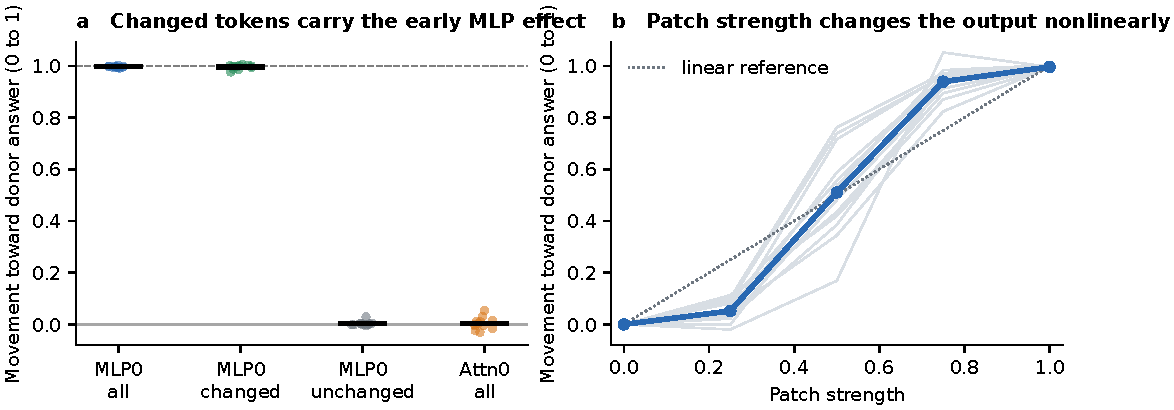
\includegraphics[width=\textwidth]{Fig1.pdf}
\caption{\textbf{Where the single-component effect comes from.}
\textbf{a}, Answer movement after copying the first MLP output at all,
changed, or unchanged positions, plus the neighboring-attention control.
\textbf{b}, Answer movement as patch strength increases. A score of 0 is the
clean recipient and 1 is the clean donor. Light marks are individual examples;
dark marks are means. Both panels show the same 12 prospectively fixed prompt
pairs in the forward direction.}
\label{fig:micro}
\end{figure}

\begin{figure}[ht]
\centering
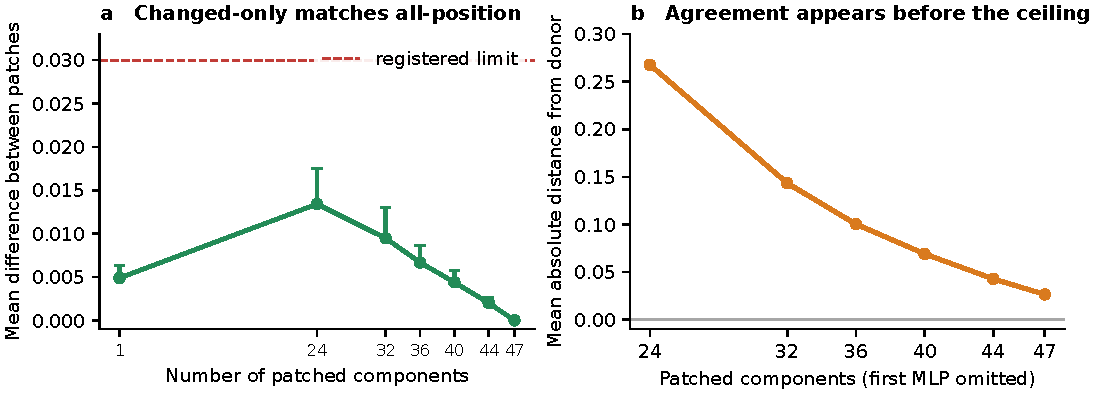
\includegraphics[width=\textwidth]{Fig2.pdf}
\caption{\textbf{Changed-position patches continue to match all-position
patches as more components are included.} \textbf{a}, Mean paired absolute
difference between the two patches for the same component sets; upper whiskers
are registered one-sided 95\% stratified-bootstrap bounds. \textbf{b}, Mean
absolute per-example distance from the donor after all-position patching,
showing that agreement appears before the output reaches a ceiling. The
one-component point uses 12 prompt pairs; the 24-, 32-, 36-, 40-, 44-, and
47-component points use 24, 16, 47, 47, 47, and 1 component sets,
respectively. Bootstrap resampling preserves matched position conditions and
resamples prompt pairs within templates; at 24--44 components it also
resamples component sets.}
\label{fig:scale}
\end{figure}

\begin{figure}[ht]
\centering
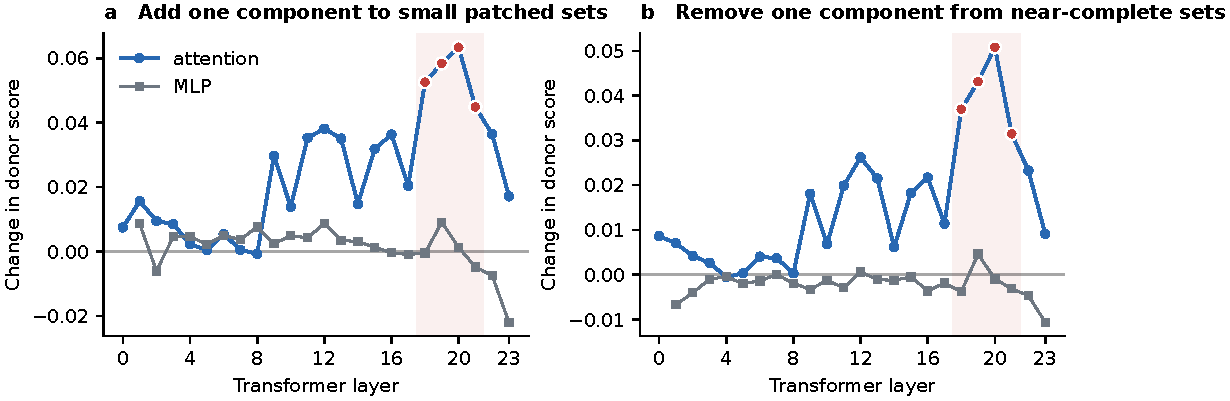
\includegraphics[width=\textwidth]{Fig3.pdf}
\caption{\textbf{Components that provide backup.} \textbf{a}, Mean score change
from adding one component to a small patched set. \textbf{b}, Score loss from
removing one component from a near-complete patched set. Points summarize 12
new prompt pairs over the fixed background sets. Blue circles are attention
outputs and gray squares are MLP outputs. Red points and shading mark attention
layers 18--21, which were suggested by earlier results and then tested on the
new examples.}
\label{fig:backup}
\end{figure}

\begin{figure}[ht]
\centering
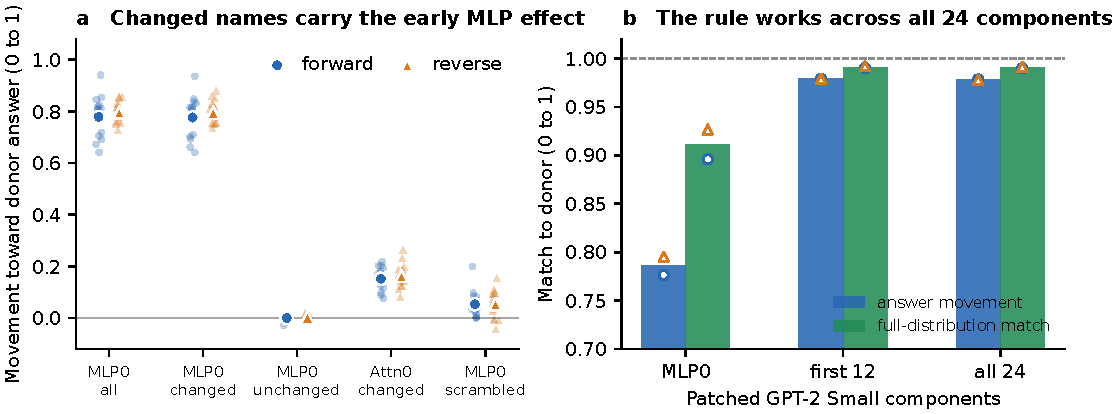
\includegraphics[width=\textwidth]{Fig4.pdf}
\caption{\textbf{GPT-2 Small indirect-object replication.}
\textbf{a}, Movement toward the donor answer after copying the first MLP
output and after negative controls. Light points are individual examples;
dark marks are means. \textbf{b}, Movement toward the donor answer and
similarity to the donor's full next-token distribution after copying changed
names through one, 12, and 24 components. Bars average the two directions;
white circle and triangle marks show the forward and reverse means. Each
direction contains the same 16 prospectively fixed prompt pairs.}
\label{fig:replication}
\end{figure}

\begin{table}[ht]
\caption{Single-component confirmation on examples fixed in advance. A score
of 0 is the clean recipient and 1 is the clean donor. The unchanged-position
column is reported in absolute value.}
\label{tab:micro}
\centering
\begin{tabular}{@{}lrrr@{}}
\toprule
Direction and component & All positions & Changed positions & Unchanged positions \\
\midrule
Forward, layer-0 MLP & 0.9963 & 0.9954 & 0.0048 \\
Reverse, layer-0 MLP & 0.9975 & 0.9945 & 0.0048 \\
Forward, layer-0 attention & \multicolumn{3}{c}{worst absolute mean $\leq 0.0172$} \\
\botrule
\end{tabular}
\end{table}

\begin{table}[ht]
\caption{Difference between changed-position and all-position patches as more
components are included. Mean gap is the mean paired absolute difference. UB
is its registered one-sided 95\% stratified-bootstrap upper bound. Donor gap is
the mean absolute per-example distance from the donor after all-position
patching.}
\label{tab:scale}
\centering
\small
\setlength{\tabcolsep}{3pt}
\begin{tabular}{@{}lrrrr@{}}
\toprule
Component set & Sets & Mean gap & 95\% UB & Donor gap \\
\midrule
24, first MLP omitted & 24 & 0.01342 & 0.01753 & 0.26780 \\
32, first MLP omitted & 16 & 0.00947 & 0.01302 & 0.14336 \\
24, first MLP included & 24 & 0.00242 & 0.00369 & 0.00251 \\
32, first MLP included & 32 & 0.00136 & 0.00171 & 0.00322 \\
36, first MLP omitted & 47 & 0.00668 & 0.00863 & 0.10032 \\
40, first MLP omitted & 47 & 0.00440 & 0.00571 & 0.06904 \\
44, first MLP omitted & 47 & 0.00201 & 0.00266 & 0.04275 \\
47, first MLP omitted & 1 & 0.00000 & 0.00000 & 0.02639 \\
\botrule
\end{tabular}
\end{table}

\end{document}
